\section{tracks.csv \& genres.csv}

The dataset "tracks" contains 106,574 tracks and 52 features while "genres" has 163 rows and 5 features. 
Tracks is partitioned in the following way: \\
$\bullet$  \textbf{Track}: stores information like listens, bit rate, duration, name of the song.\\
$\bullet$ \textbf{Artist}: contains information about the name of the artist, location and members of the band.\\
$\bullet$ \textbf{Album}: provides specific information about each single album (i.e. years created, name).\\
The dataset collects songs from 2008 to 2018. In Figure 1.1 we show the number of tracks and album published along the years.

\begin{figure}[hp]
  \centering
  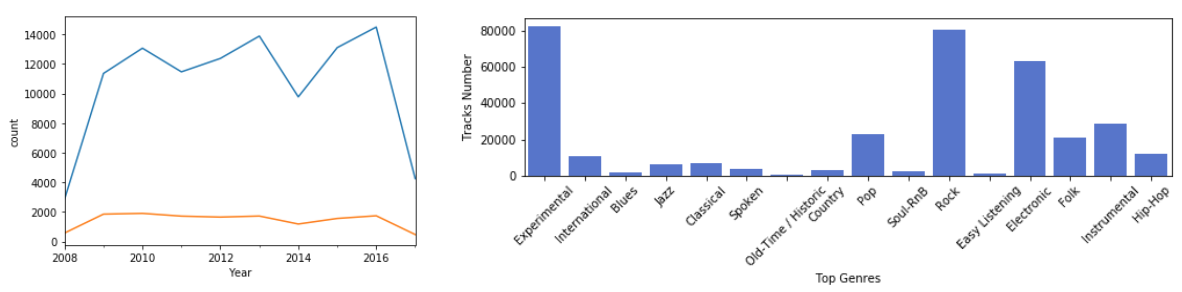
\includegraphics[width=0.9\linewidth]{images/year_tracks-genre-per-track.png}
  \caption{On the left we plot the number of tracks (blue line) and of album (orange line} per year. On the right we show the number of tracks available per (top) genre.
\end{figure} 



Some features have less than 1\% of available data, therefore they were discarded. The most significant ones did not contain missing values, except for \textit{"genre\_top"} which had 46.54\% of available data. In order to replace the missing values we first tried to exploit the information provided in the dataset \textit{"genre.csv"}. By doing so, we discovered that songs with missing \textit{"genre\_top"} label, were those for which a track was labelled with more than one genre. Some tracks were assigned more than 10 different genres, therefore it was difficult to identify the most appropriate one. Since the 46.54\% of \textit{"genre\_top"} provided us a sufficient amount of data to carry out the analysis, we decided to disregard the tracks for which the \textit{"genre\_top"} label was \textit{Null}. 

We noticed that the bit rate was expressed in bits per second. Since this value was considerably high w.r.t. to the other data, we re-scaled it in kilo-bit per second (scaled down by a factor of 1000).
Majority of the tracks have a bit rate between 250 and 350 kbps.

On average tracks have a duration of 277 seconds. The distribution is slightly left skewed with a std of 305.51. This is a clear signal that our data might contained outliers, as some of the data have a duration of almost 1.5 std greater than the mean. Analysing instead the distribution of the attribute \textit{"listens"}, we observed that it is highly left-skewed with less than 1,000 tracks having more than 2,000 listens. On average a track has 2,329 listens, even though this values is highly influenced by few "potential outliers" having around 5000 listens per track. 

% Need to be changed with the one with highest resolution. cannot read the nubmers on the graph
\begin{figure}[hp]
  \centering
  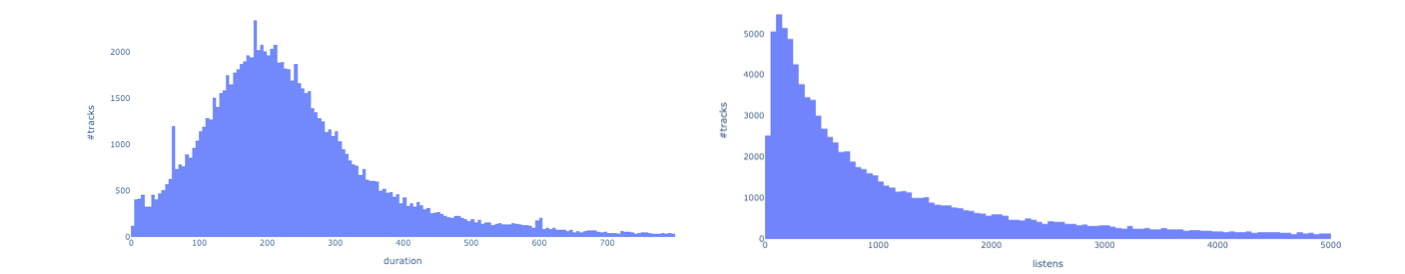
\includegraphics[width=1.01\linewidth]{images/duration-listens_tracks.csv.png}
  \caption{On the left we plot the distribution of the \textit{"duration"} of a song. On the right we show the number of listens per track.}
\end{figure} 

Experimental, Rock and Electronic are the genres for which there are more artists ( 2,609, 2,065 and 2,050 respectively). These 3, have also the highest number of tracks in the dataset (as shown in Figure 1.2). Regarding the geographical origin of the songs, we exploited the latitude and longitude provided in echonest.csv to discovered that most of them are American and European, with very few songs produced in Asia.
The dataset includes songs belonging to 163 genres, which can be grouped in 16 top genres. For the analysis we decided to work only with a subset of those.

\section{features.csv}

The dataset consists of 106,574 tracks and 518 features. The dataset appears clean, as there are no missing values. However, we detected 2,111 duplicates which were properly removed.
The attributes provided in this partition, were extracted using the Librosa library, which translated the spectrograms of each song into continuous values.
The main features extracted are: \\
$\bullet$ \textbf{mfcc}: these features are useful for recognizing the timbre of a song.\\
$\bullet$ \textbf{chroma}: are able to capture armonic and melodic characteristics of a song. \\
$\bullet$ \textbf{tonnetz}: represents the tonal space.\\
$\bullet$ \textbf{spectral} (roll-off, contrast, centroid, bandwidth): describes the frequency and the energy of a song. \\
$\bullet$ \textbf{zrc}: rate at which a signal changes from positive to zero to negative or vice-versa. It is useful for recognising percussive sounds.\\

\section{echonest.csv}
The dataset contains 13,129 rows and 249 features. It is partitioned into \textit{"echonest\_audiofeatures"} (\textit{acousticness, danceability, energy, instrumentalness, liveness, speechiness, tempo, valence}), \textit{"metadata"} (general information about a song, like album name etc.) and \textit{"temporal features"}. 
The features provided in the first partition have a values in range [0, 1]. To better understand the characteristics of each genre, we plotted a radar chart, which highlights their differences. Below we show only few of the visualizations that were made. 
\begin{figure}[hp]
  \centering
  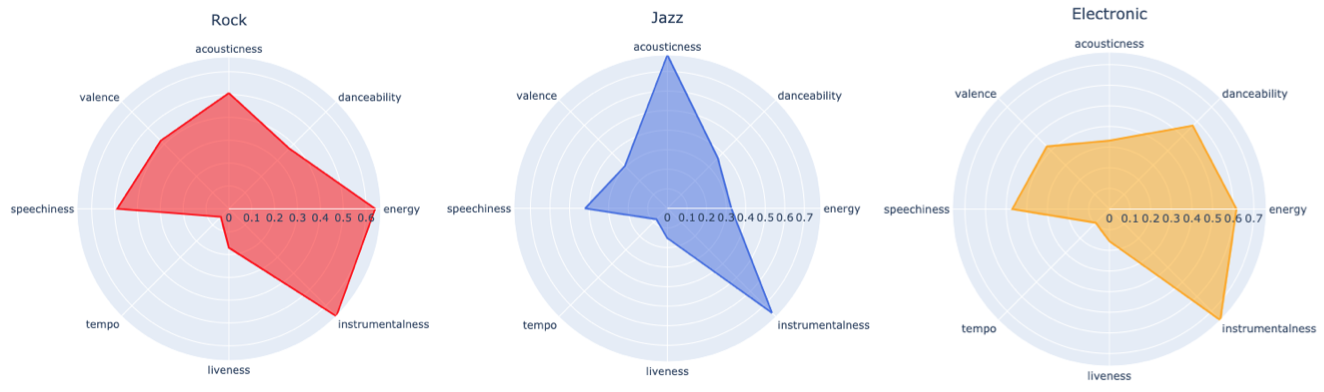
\includegraphics[width=0.85\linewidth]{images/radar-plot_Rock-Jazz-Electronic.png}
  \caption{Radar chart of echonest audio-features for Rock, Jazz and Electronic.}
\end{figure} 

We also researched the meaning of each of those features, and useful information that helped us in defining the tasks. For example \textit{"liveness"} indicated whether a song was recorded during a live concert or in a studio, "valence" referred to the happiness of a song, and \textit{"instrumentalness"} indicated the ratio between words in a song and instruments played. Analyzing the values of the latter, we trivially discovered some potential outliers (which will be detected in the following sections). In fact some tracks had an instrumentalness very close to 0 ( meaning the tracks was composed of just words) and in combination with the information provided by the attribute "duration", we assessed that those tracks were not "real songs", but merely intros of an album, as their duration did not exceed 18 seconds.\\
The partition \textit{"social features"} provided us information extracted from statistics about song hotness, artist familiarity and others. These were used to create the task of "Song popularity classification", which will be briefly described in the next sections. 
